\section{The \flare\ Simulations}
\label{sec:method}

\begin{figure}
	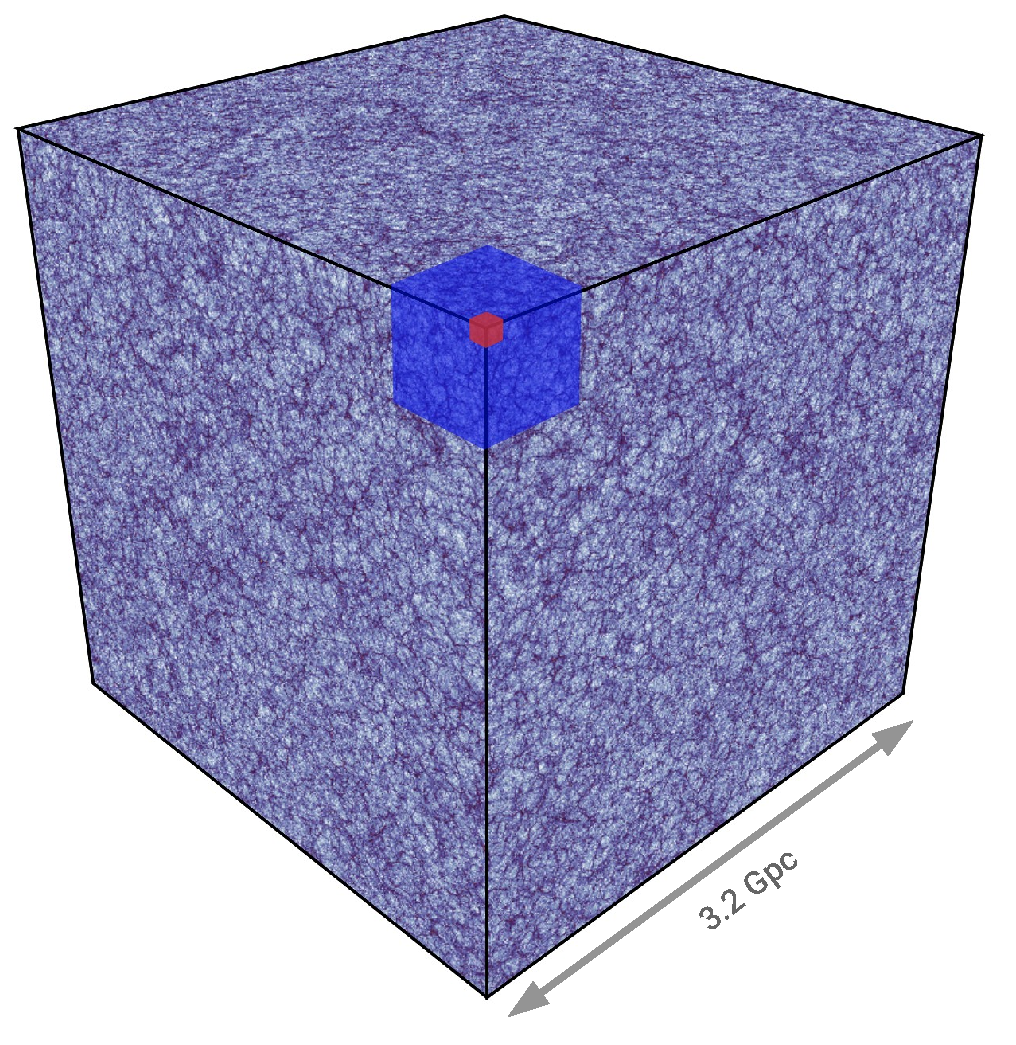
\includegraphics[width=\columnwidth]{images/parent_box.pdf}
    \caption{Diagram of the 3.2\,cGpc box from which we select our regions \citep{barnes_redshift_2017}.
		To demonstrate the increase in volume, we show the Bluetides simulation \protect\citep[$L = 570$\,cMpc;][]{feng_bluetides_2016} inset in blue, and the fiducial EAGLE simulation \protect\citep[$L = 100$\,cMpc;][]{schaye_eagle_2015} inset in red.}
    \label{fig:L3200}
\end{figure}

We will now detail our simulations, including the selection of the regions and the zoom resimulation technique.
Full details of the \eagle\ physics model are provided in \cite{schaye_eagle_2015,crain_eagle_2015}.

\subsection{Region Selection}
\label{sec:method:region}

We use the same parent simulation as that used in the \ceagle\ simulations \citep{barnes_redshift_2017}: a (3.2\,cGpc)$^3$ dark matter-only simulation with a particle mass of $8.01 \,\times\, 10^{10}$\,\Msun, using the \cite{planck_collaboration_planck_2014} cosmology.
\fig{L3200} shows a diagram of the box compared to the fiducial \eagle\ reference volume, as well as the \bluetides\ simulation \citep{feng_bluetides_2016}.
The highest redshift snapshot available for this simulation is at $z = 4.67$, which we use for our selection.
Within this snapshot, we select spherical volumes that sample a range of overdensities.
By taking a sufficiently large radius we can ensure that the density fluctuations averaged on that scale are linear, such that the distortion in the shape of the Langrangian volume during the simulation will not be too extreme and that the ordering of the density fluctuations is preserved.
The regions, and their overdensities, are given in \tab{regions}.

\begin{figure}
  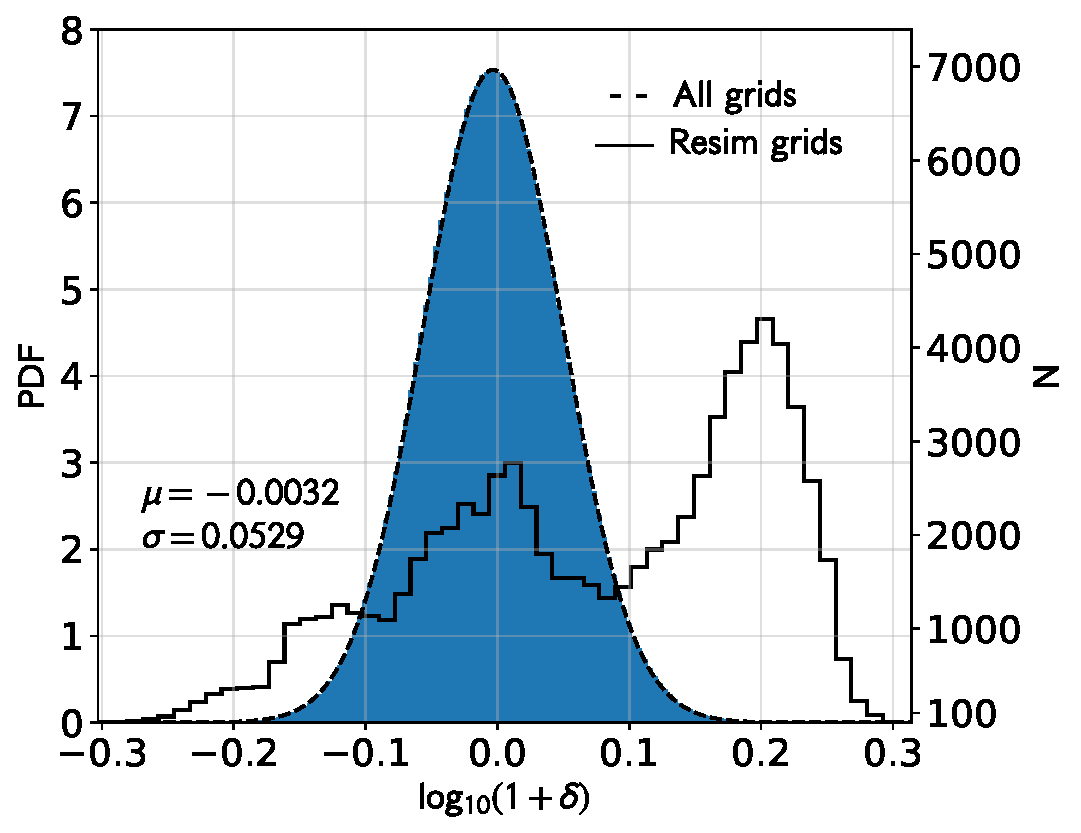
\includegraphics[width=\columnwidth]{images/sampling_bins.pdf}
  \hspace*{0.15cm}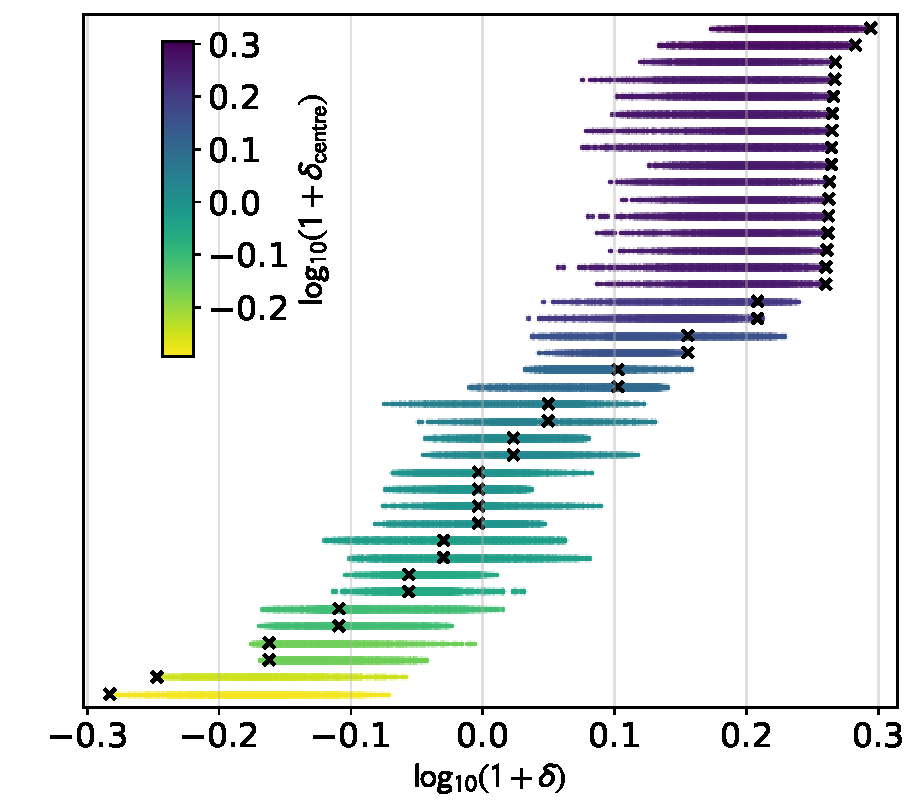
\includegraphics[width=0.85\columnwidth]{images/cum_delta.pdf}
  \caption{\textit{Upper panel}: the probability distribution function of sampled overdensities.
	The dashed black line shows a lognormal fit with the given parameters.
	The solid blue histogram shows the grid locations that lie within one of our resimulation volumes.
	The solid black histogram shows the distribution of our selected regions in overdensity, binned into 50 equal width bins, with the right y-axis showing only their number counts.
	\textit{Lower panel}: the distribution of over-densities within each simulation volume. The vertical displacement is arbitrary.  The cross shows the overdensity measured at the centre of the resimulated volume and the spread of values shows the overdensities within each volume evaluated at each point on the 2.67\,cMpc grid.}
  \label{fig:log_fit}
\end{figure}

To determine the density, we first distribute the mass onto a high resolution, $3.2 \; \mathrm{cGpc}\,/\,1200 \sim 2.67\; \mathrm{cMpc}$ cubic grid using a nearest grid point assignment scheme.
We then find the density on larger scales by convolving the grid with a spherical top-hat filter of radius $14$ \cMpch.\footnote{Code provided at \\\href{https://github.com/christopherlovell/DensityGridder}{https://github.com/christopherlovell/DensityGridder}}
We find, in test volumes, that this gives densities very close to those calculated from the raw particle data.
The overdensity is then defined as
\begin{equation}\label{eq:1}
	\delta(\textbf{x}) = \frac{\rho(\textbf{x})}{\bar\rho} - 1,
\end{equation}
where $\rho$ is the density at grid coordinates $\textbf{x}$, and $\bar\rho$ is the mean density in the box.
The upper panel of \fig{log_fit} shows the distribution of overdensity in log-space, alongside a fitted log-normal distribution.

We select regions for resimulation with two different goals: firstly, we select a number of regions of high overdensity in order to obtain a large sample of the first massive galaxies to form in the Universe; and secondly we select regions with a range of overdensities in order to explore the environmental impact (bias) on galaxy formation.
The selected regions are listed in \app{regions} and the range of overdensities that each covers (evaluated at each point on the 2.67\,cMpc grid enclosed by that volume) is shown in the lower panel of \fig{log_fit}.
We discuss how to combine the resimulations so as to obtain a representative sample of the whole Universe in \Sec{method:weighting}.


\subsection{The resimulation method}
\label{sec:method:resim}

\begin{table}
	\centering
	\caption{Variation of subgrid parameters between models. }
	\label{tab:example_table}
	\begin{tabular}{lcccc}
		\hline
		\textbf{Simulation Prefix} & $C_{\mathrm{visc}}$ & $\Delta T_{\mathrm{AGN}}$\\
		\hline
      & & $\mathrm{[K]}$ \\
		\hline
		Ref & $2 \pi$ & $10^{8.5}$ \\
		AGNdT9 & $2 \pi \times 10^{2}$ & $10^{9}$ \\
		\hline
	\end{tabular}
\end{table}


\begin{figure*}
  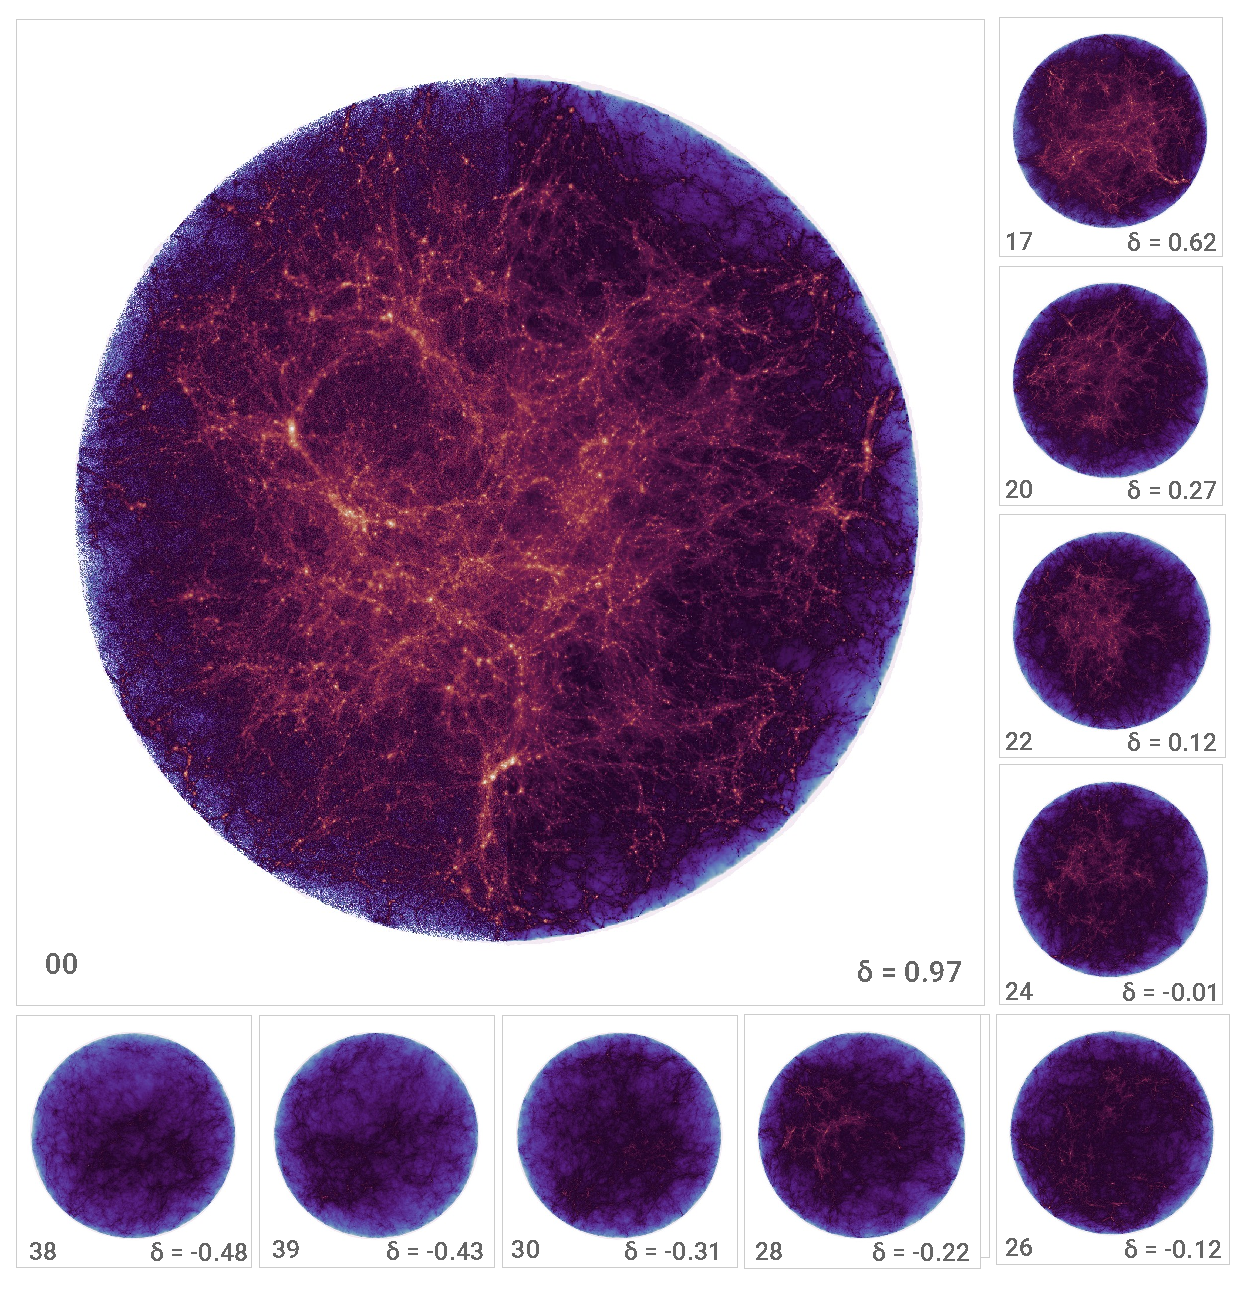
\includegraphics[width=\textwidth]{images/flares_regions.pdf}
  \caption{Visualisation of the dark matter integrated density in the periodic fiducial \eagle\ volume compared to two \flares\ regions at $z = 5$.
	The periodic box shows a slice of width ???.
	The resimulation regions show the whole high-resolution region.
	We show a high density region and a low density region to demonstrate the range of environments sampled in \flares.
	}
  \label{fig:sm_vis}
\end{figure*}


We use the AGNdT9 configuration of the \eagle\ parameters, as described in \citet{schaye_eagle_2015}, which produces similar mass functions to the reference model but better reproduces the hot gas properties in groups and clusters \citep{barnes_cluster-eagle_2017}.
This is identical to that used in the \ceagle\ simulations, but differs from the fiducial Reference simulation (see \tab{example_table}).
It uses a higher value for $C_{\mathrm{visc}}$, which controls the sensitivity of the BH accretion rate to the angular momentum of the gas, and a higher gas temperature increase from AGN feedback, $\Delta T$.
A larger $\Delta T$ leads to fewer, more energetic feedback events, whereas a lower $\Delta T$ leads to more continual heating.
We use an identical resolution to the fiducial \eagle\ simulation, with gas particle mass $m_{g} = 1.8 \times 10^6 \; \mathrm{M_{\odot}}$, and a softening length of $2.66 \; \mathrm{ckpc}$.

Galaxies on the edge of the high resolution region will not be modelled correctly due to the presence of a pressureless boundary.
To avoid this we resimulate a region 15\,\cMpch\, in radius, and ignore all galaxies within 1\,\cMpch\, of the edge of the sphere in post-processing.
At higher redshift the lagrangian high resolution region can deform, but we found that it is close to spherical out to the highest redshifts considered in this work ($z = 10$).
\fig{sm_vis} shows the dark matter distribution within the cutout radius for a range of resimulations of differing overdensity, at $z = 4.7$.
We also show the fiducial periodic \eagle\ volume to provide a visual comparison of the differing environments probed.

As in the standard \eagle\ analysis, structures are first found using a Friends-Of-Friends \citep[FOF,][]{davis_evolution_1985} finder, then split into bound galaxy substructures using the \textsc{Subfind} algorithm \citep{springel_populating_2001}.
Their properties are then defined using those stellar particles within 30\,pkpc of the location of the most tightly-bound stellar particle.
We limit our analysis to galaxies sampled by at least 50 star particles, which corresponds to a mass limit of approximately $\mathrm{log_{10}(M_{*}\,/\,M_{\odot})} \geqslant 7.95$.
We assume a Chabrier IMF throughout \citep{chabrier_galactic_2003}.

\subsection{Distribution Function Weighting}
\label{sec:method:weighting}

In this section we describe how we combine our resimulations to obtain a statistically-correct representation of the universal cosmological distribution of galaxies.
As we show below in \Sec{results:gsmf}, distribution functions, such as the galaxy stellar mass function, vary with the overdensity of the resimulated volume.
It is therefore necessary to \textit{weight} each resimulation to reproduce the correct distribution of those overdensities averaged over the whole universe, i.e. the cosmic mean.

As mentioned in \Sec{method:region}, the overdensity within spherical top-hat regions of radius 14\,\cMpch\, is sampled on a 2.67\,cMpc grid; we label this sample $\delta_g$.
Since the grid sampling is finer than the size of the resimulation volume, each resimulation volume is associated with just under 2000 different values of $\delta_g$.
We show the distribution of those $\delta_g$ within each resimulation volume in the lower panel of \Fig{log_fit}.
The most overdense regions, whilst containing a single highly overdense point, in fact contain points covering a range of overdensities.
It is therefore important to account for this spread in sampled overdensity, rather than just using the central overdensity when determining the contribution from any particular resimulation volume.
% This shows that, while our resimulations span the full range of overdensities, they do not fairly sample the cosmic mean: indeed, we have deliberately concentrated on overdense regions where the most luminous galaxies are located.

The top panel of \Fig{log_fit} contrasts the PDFs of $\delta_g$ for the whole box and for our resimulated sample.
To generate the correct mean distibutions, we divide into bins of overdensity as shown by the histogram in \fig{log_fit} (black solid line), then \textit{weight} the resimulations appropriately to reproduce the cosmic distribution.
Specifically, we do the following:
\begin{itemize}
\item The overdensity domain is split up into 50 bins of equal width in $\log_{10}(1+\delta)$, $i=1 \ldots N_\delta$.\footnote{We tested using a greater number of bins and found that the quantitative weights did not change significantly.}
For each of these, it is possible to assign a weight, $w_{\mathrm{true},i}$, in proportion to the fraction of $\delta_g$ that lie in that bin, such that $\Sigma_iw_{\mathrm{true},i}=1$.
\item Each resimulation, $j$, is similarly distributed over these overdensity bins with weights, $w_{ij}$, in proportion to the enclosed values of $\delta_g$.  Thus $\Sigma_iw_{ij}=1$.
\item The sample weight associated with each bin is $w_{\mathrm{sample},i}=\Sigma_jw_{ij}$.
\item To obtain the correct universal average, we therefore have to weight each density bin by the ratio $r_i=w_{\mathrm{true},i}/w_{\mathrm{sample},i}$.
\end{itemize}
Ideally, we would associate each galaxy with the local value of $\delta_g$.
However, for the purposes of simplicity in this paper, we give all galaxies within a particular resimulation equal weight -- this will give some dispersion over the more correct method, which we will implement in a future paper.
\begin{itemize}
\item Hence we adjust the contribution of each resimulation by a factor $f_{j}=\Sigma_ir_iw_{ij}$.
\end{itemize}
We note that
\begin{align}
  \Sigma_j f_j &= \Sigma_j \Sigma_i r_i w_{ij} = \Sigma_i r_i \Sigma_j w_{ij} \nonumber \\
  &= \Sigma_i r_i w_{\mathrm{sample},i} = \Sigma_i w_{\mathrm{true},i} =1.
\end{align}
These simulation weighting factors are listed in \Tab{regions}.

We further note that, at higher redshifts, the overdensities will evolve.
Nevertheless, because even the most extreme perturbations are only mildly non-linear, we would expect that the ordering of the overdensities would largely be preserved.
Hence we use the same sampling at all redshifts.
That also allows for a much more direct comparison of the evolution within each overdensity sample.
